% This file was converted to LaTeX by Writer2LaTeX ver. 1.0.2
% see http://writer2latex.sourceforge.net for more info
\documentclass[letterpaper]{article}
\usepackage[ascii]{inputenc}
\usepackage[T1]{fontenc}
\usepackage[english]{babel}
\usepackage{amsmath}
\usepackage{amssymb,amsfonts,textcomp}
\usepackage{color}
\usepackage{array}
\usepackage{hhline}
\usepackage{hyperref}
\hypersetup{pdftex, colorlinks=true, linkcolor=blue, citecolor=blue, filecolor=blue, urlcolor=blue, pdftitle=, pdfauthor=pavan, pdfsubject=, pdfkeywords=}
\usepackage[pdftex]{graphicx}
% Page layout (geometry)
\setlength\voffset{-1in}
\setlength\hoffset{-1in}
\setlength\topmargin{2.399cm}
\setlength\oddsidemargin{2.364cm}
\setlength\textheight{25.047cm}
\setlength\textwidth{16.968cm}
\setlength\footskip{0.0cm}
\setlength\headheight{0cm}
\setlength\headsep{0cm}
% Footnote rule
\setlength{\skip\footins}{0.119cm}
\renewcommand\footnoterule{\vspace*{-0.018cm}\setlength\leftskip{0pt}\setlength\rightskip{0pt plus 1fil}\noindent\textcolor{black}{\rule{0.25\columnwidth}{0.018cm}}\vspace*{0.101cm}}
% Pages styles
\makeatletter
\newcommand\ps@Convertedi{
  \renewcommand\@oddhead{}
  \renewcommand\@evenhead{}
  \renewcommand\@oddfoot{}
  \renewcommand\@evenfoot{}
  \renewcommand\thepage{\arabic{page}}
}
\newcommand\ps@Standard{
  \renewcommand\@oddhead{}
  \renewcommand\@evenhead{}
  \renewcommand\@oddfoot{}
  \renewcommand\@evenfoot{}
  \renewcommand\thepage{\arabic{page}}
}
\newcommand\ps@Convertediii{
  \renewcommand\@oddhead{}
  \renewcommand\@evenhead{}
  \renewcommand\@oddfoot{}
  \renewcommand\@evenfoot{}
  \renewcommand\thepage{\arabic{page}}
}
\newcommand\ps@Convertedii{
  \renewcommand\@oddhead{}
  \renewcommand\@evenhead{}
  \renewcommand\@oddfoot{}
  \renewcommand\@evenfoot{}
  \renewcommand\thepage{\arabic{page}}
}
\makeatother
\pagestyle{Standard}
\title{}
\author{pavan}
\date{2013-11-18}
\begin{document}
\clearpage\setcounter{page}{1}\pagestyle{Standard}
{\selectlanguage{english}
\textbf{III}\textbf{.}\textbf{ }\textbf{S}\textbf{ONAR}}

\begin{center}
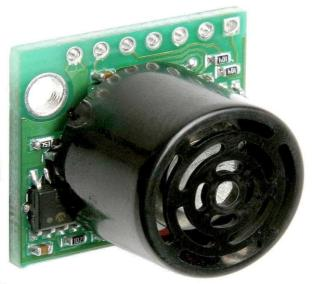
\includegraphics[width=3.968cm,height=3.624cm]{III-img1.png}
\end{center}

\bigskip

{\selectlanguage{english}
Sonar (Sound Navigation and Ranging) \ is a technique that \ uses sound
propagation (usually underwater, as in submarine navigation) to
navigate, communicate with or detect objects on or under the surface of
the water, such as other vessels. Two types of technology share the
name {\textquotedblleft}sonar{\textquotedblright}: passive sonar is
essentially listening for the sound made by vessels; active sonar is
emitting pulses of sounds and listening for echoes. Sonar may be used
as a means of acoustic location and \ of measurement \ of the echo
\ characteristics of {\textquotedblleft}targets{\textquotedblright} in
the water. Acoustic location in air was used before the introduction of
radar. Sonar may also be used in air for robot navigation, and SODAR
(upward looking in{}-air sonar) is used for atmospheric
investigations.}


\bigskip

{\selectlanguage{english}
The term sonar is also used for the equipment used to generate and
receive the sound. The acoustic frequencies used in sonar systems vary
from very low (infrasonic) to extremely high (ultrasonic). The study of
underwater sound is known as underwater acoustics or hydro acoustics.}


\bigskip


\bigskip


\bigskip

{\selectlanguage{english}
\textbf{i. }\textbf{\ }\textbf{S}\textbf{o}\textbf{n}\textbf{ar}\textbf{
}\textbf{S}\textbf{e}\textbf{n}\textbf{s}\textbf{i}\textbf{ng}}


\bigskip

{\selectlanguage{english}
Sonar or \ ultrasonic \ sensing \ uses \ propagation \ of acoustic
energy \ at \ higher \ frequencies than normal \ hearing \ to \ extract
\ information \ from \ the \ environment. \ Sonar \ is \ a \ popular
\ sensor \ in robotics that employs acoustic pulses and their echoes to
measure range to an object. Since the sound \ speed \ is usually known,
\ the object \ range is proportional to \ the echo \ travel time. At
ultrasonic frequencies the sonar energy is concentrated in a beam,
providing directional information in addition to range.}


\bigskip

{\selectlanguage{english}
Its popularity is due to its inexpensive cost, light weight, low power
consumption, and low computational effort, compared to other ranging
sensors. In some applications, such as in underwater and
low{}-visibility environments, sonar is often the only viable sensing
modality.}


\bigskip

{\selectlanguage{english}
Sonars in robotics have three different, but related, purposes:}


\bigskip

{\selectlanguage{english}
(a) Obstacle avoidance: The first \ detected echo \ is assumed to
\ measure the range to the closest object. Robots use this information
to plan paths around obstacles and to prevent collisions.}

{\selectlanguage{english}
(b) Sonar \ Mapping: \ Sonar \ mapping: \ A \ collection \ of \ echoes
\ acquired \ by \ performing \ a rotational scan or from a sonar array,
are used to construct a map of the environment. Similar to a radar
display, a range dot is placed at the detected range along the probing
pulse direction.}

{\selectlanguage{english}
(c) Object recognition: A sequence of echoes or sonar maps are processed
to classify echo producing structures composed of one or more physical
objects. When successful, this information is useful for robot
registration or landmark navigation.}

\clearpage\setcounter{page}{1}\pagestyle{Convertedi}
{\selectlanguage{english}
Some of the famous companies which manufacture sonar sensors are
Parallax and Maxbotix. Maxbotix \ provides \ a range \ of 60 \ sensors
along \ 12 \ product \ lines \ which \ vary \ based \ on the
environment, precision, beam width and connection module.}


\bigskip

{\selectlanguage{english}
One of the most sought of series is the LV series because of its high
precision, robustness, programming simplicity and ease in connection.
Various libraries are available for Arduino and other development
boards. The only drawback of this series is the resolution (1 inch)
which cannot be used where high accuracy is required.}


\bigskip

 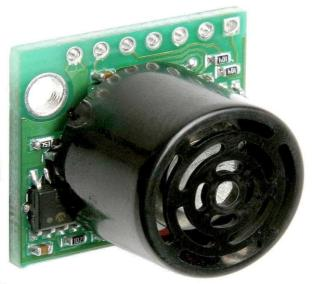
\includegraphics[width=3.969cm,height=3.625cm]{III-img2.png} 


\bigskip


\bigskip


\bigskip


\bigskip

{\selectlanguage{english}
The HR series is the series which gives the highest resolution. They can
be connected via USB or direct connection and can be used in indoor as
well as outdoor environment. The Maxsonar sensors give both digital and
analog reading and can be easily read and converted to distance using
some basic formulae. The Maxsonar sensors can also be used for people
detection and height detection. One of the most important advantages of
Maxbotix sensors is that they can be daisy chained. Daisy chaining is a
technique to connect one or more devices together and avoid
interference between them. The Maxsonar Sensors can be daisy chained in
3 different ways {}-- the free run mode, the commanded loop
mode(software triggered) and the continuous loop mode(hardware
triggered).}


\bigskip

{\selectlanguage{english}
The sonars belonging to the LV Series have 7 pins and can give both
analog and digital output. They can operate at 3.3V and 5V. They also
have a pin for series chaining.}


\bigskip

{\selectlanguage{english}
(a) Analog Output}

{\selectlanguage{english}
The analog output from the LV Sonar can be obatined from the AN pin of
the Sonar. \ The voltage}

{\selectlanguage{english}
output is from 0 to Vcc/2 . The resolution of the sonar is 512. This
resolution should be taken care of when taking the sonar readings on a
microcontroller having a differnet resolution.}


\bigskip

{\selectlanguage{english}
(b) Digital Output}

{\selectlanguage{english}
The Digital Output can be measured from the PW pin of the Sonar.
Whenever the Sonar starts ranging, the PW pin pulled HIGH. Whenever a
target is detected, the PW pin is pulled low. The time for which the PW
pin is high can be calculated using the pulseIn() function on an
Arduino and the distance to the obstacle can be calculated.}

\clearpage\setcounter{page}{1}\pagestyle{Convertedii}
{\selectlanguage{english}
(c) Daisy Chaining:}

{\selectlanguage{english}
For low noise chaining the BW pin of the sonar has to be pulled high.
The chaining can be three}

{\selectlanguage{english}
types:}


\bigskip

{\selectlanguage{english}
The free run mode, where multiple sonars are ranging continously. This
method is to be avoided because it can cause interference between
multiple sound waves and give false results.}


\bigskip

{\selectlanguage{english}
The chain can be controlled by software using a software controlled
loop. The RX of the first sonar \ is \ connected \ to \ a \ digital
\ output \ pin \ on \ the \ microcontroller. The TX \ of \ nth \ sonar
\ is connected to RX of (n+1)th sonar and the RX of first sonar is
trigered by atleast a 20us long pulse for all sonars to range once. For
every cycle, the RX has to triggered to take the readings from the
sonars}


\bigskip

{\selectlanguage{english}
The hardware controlled loop is similar to the software controlled loop.
The only difference is that the TX of the last sonar is conencted to
the RX of the first sonar by a 1K resistor and the RX of the first
SONAR needs to be triggered only once. The cycle continues till power
is supplied and readings can be taken continuously.}


\bigskip

{\selectlanguage{english}
The time from which a SONAR is triggered to the time taken for one
ranging cycle is 50ms. So the frequency of readings when one sonar is
used is 1s/50ms = 20 . This frequency reduces with increase in the
number of sonars. So frequency reduces during daisy chaining.}


\bigskip


\bigskip


\bigskip


\bigskip


\bigskip


\bigskip


\bigskip

{\selectlanguage{english}
Our usage: we are using this sonar because it gives a digital output
which I can use directly without doing any complicated computations. We
can know \ the distance of the nearest object. By setting optimum
threshold values \ we will know if the objects are obstacles or not.}

\clearpage\setcounter{page}{1}\pagestyle{Convertediii}

\bigskip
\end{document}
